% source: https://git.fslab.de/mmklab/latex-templates/tree/master/presentation

\documentclass[10pt]{beamer}

%\useoutertheme{progress}

\usepackage{etoolbox}
\newtoggle{german}

% % % % % LANGUAGE % % % %
% Make your choice here
\togglefalse{german} % English
%\toggletrue{german} % German
% % % % % \LANGUAGE % % % %

% % % Handouts % % %
%\usepackage{handoutWithNotes}
%\pgfpagesuselayout{2 on 1 with notes landscape}[a4paper,border shrink=5mm]
% % % Handouts % % %


\iftoggle{german}{
\usepackage[ngerman]{babel} % Deutsche Sprachanpassungen
\usepackage[T1]{fontenc}    % Silbentrennung bei Sonderzeichen
\usepackage[utf8]{inputenc} % Direkte Angabe von Umlauten im Dokument.Wenn Sie an einem Mac sitzen,verwenden Sie ggf. „macce“ anstatt „utf8“.
\usepackage[autostyle=true,german=quotes]{csquotes} % Anfuehrungszeichen\
}{
\usepackage[utf8]{inputenc}}

\usepackage[utf8]{inputenc}
\usepackage[T1]{fontenc}
\usepackage{textcomp}
% \setbeamercovered{transparent} %Useful for maintaining transparent next point while using <1- >
\usepackage{default}
\usepackage{lmodern}
\usepackage{amsmath,amsfonts,amssymb} % Mathe
\usepackage{eurosym}
\usepackage{tikz}
\usepackage{graphicx}
%\usepackage[labelformat=empty]{caption}
\usepackage{verbatim}
\usepackage{color}
\usepackage{hypernat}
\usepackage{tabularx}
\usepackage[]{units}
\usepackage{caption}
\usepackage{comment}
%\usepackage{subfigure}
\usepackage{wasysym}
\usepackage{ulem}
\usepackage[printonlyused]{acronym} 
\usepackage{tabularx}
\usepackage{appendixnumberbeamer}
\usepackage{epigraph}
\usepackage{remreset}% tiny package containing just the \@removefromreset command
\usepackage{subcaption}
\usepackage{makecell}
\usepackage{pdfpcnotes}% Usefull package for notes for presentations
\usepackage{colorbar}
%\usepackage{./progbar}
%\usepackage{./beamerouterthemeprogress}
\usepackage{hyperref}
\usepackage[ruled,vlined]{algorithm2e}
\usepackage{multirow}

\let\Tiny=\tiny % Reduces a few recent error on Unix systems

\usepackage[sorting=none,style=numeric-comp,backend=bibtex]{biblatex} % load the package
\addbibresource{./bibliography.bib} % Add your bib file
\renewcommand*{\bibfont}{\footnotesize}

% % % % Style % % % %
% Some colours as used in other programms like openoffice
\definecolor{red}{RGB}{184,71,71}
\definecolor{green}{RGB}{51,204,102}
\definecolor{blue}{RGB}{0,153,255}
\definecolor{fhblau}{rgb}{0, 0.594, 0.949}

\setbeamercolor{title}{bg=fhblau, fg=white}
\setbeamercolor{frametitle}{bg=fhblau, fg=white}
\setbeamercolor{structure}{fg=fhblau}

% MISC Styles %
\setbeamertemplate{bibliography item}[text]
\usetheme{default}
\setbeamertemplate{footline}[frame number]
\setbeamertemplate{caption}[numbered]
\setbeamersize{text margin left=0.3cm,text margin right=0.3cm}
\setbeamertemplate{navigation symbols}{}%remove navigation symbols
\makeatletter
\@removefromreset{subsection}{section}
\makeatother
\setcounter{subsection}{1}


% Here are some usefulf different fonts. Use them in every flooting enviroment with \usebeamerfont{AAA}
\setbeamerfont{AAA}{size*={16.00}{15.00}}
\setbeamerfont{aaa}{size*={12.00}{11.00}}
\setbeamerfont{bbb}{size*={11.00}{11.00}}
\setbeamerfont{ccc}{size*={10.00}{11.00}}
\setbeamerfont{ddd}{size*={9.00}{11.00}}
\setbeamerfont{eee}{size*={8.00}{11.00}}
\setbeamerfont{fff}{size*={7.75}{10.75}}
\setbeamerfont{ggg}{size*={7.50}{10.50}}
\setbeamerfont{hhh}{size*={7.25}{10.25}}
\setbeamerfont{iii}{size*={7.00}{10.00}}
\setbeamerfont{jjj}{size*={6.00}{9.00}}
\setbeamerfont{kkk}{size*={5.00}{8.00}}
\setbeamerfont{lll}{size*={4.00}{7.00}}
\setbeamerfont{mmm}{size*={3.00}{6.00}}
\setbeamerfont{nnn}{size*={2.00}{5.00}} 
% Set some beamer fonts


\setbeamerfont{title}{size=\Large,series=\bfseries,parent=structure}
\setbeamerfont{caption}{size=\footnotesize}
\setbeamertemplate{footline}[text line]{%
	\parbox{\linewidth}{\vspace*{-8pt}\hspace{1em}\insertshortauthor\hspace{10mm} 
	Towards Smart Coupling in Multiphysics Simulation
	\hfill\insertframenumber/\inserttotalframenumber}} 

\renewcommand*{\bibfont}{\usebeamerfont{kkk}}

% A new cell type
\newcommand{\specialcell}[2][c]{%
  \begin{tabular}[#1]{@{}c@{}}#2\end{tabular}}

% This is useful if you want to use enumerations over several frames
\newcounter{saveenumi}
\newcommand{\seti}{\setcounter{saveenumi}{\value{enumi}}}
\newcommand{\conti}{\setcounter{enumi}{\value{saveenumi}}}

\AtBeginSection[]{
  \begin{frame}[plain,noframenumbering]
      %\addtocounter{framenumber}{-1}
  \vfill
  \centering
  \begin{beamercolorbox}[sep=8pt,center,shadow=true,rounded=true]{title}
    \usebeamerfont{title}\insertsectionhead\par%
  \end{beamercolorbox}
  \vfill
  \end{frame}
}

\iffalse
\AtBeginSection[]{
  \begin{frame}[plain]{Table of Contents}
  	\tableofcontents[currentsection, hideallsubsections]
   	\addtocounter{framenumber}{-1}
  \end{frame}
}
\fi

\makeatletter
\newcommand\titlegraphicii[1]{\def\inserttitlegraphicii{#1}}
\titlegraphicii{}
\setbeamertemplate{title page}
{
  \vbox{}
  \begin{centering}
	\begin{minipage}{.8\textwidth}
	\begin{beamercolorbox}[sep=8pt,center]{title}
	  \usebeamerfont{title}\inserttitle\par
	\end{beamercolorbox}%
	\end{minipage}
	\vskip1em\par
	\begin{minipage}{.45\textwidth}
    \begin{beamercolorbox}[sep=8pt,center]{title}
	  \Large R\&D Defense\par
	\end{beamercolorbox}%
	\vskip1em\par
	\end{minipage}
	\begin{beamercolorbox}[sep=8pt,center]{author}
	  \usebeamerfont{author}\insertauthor \par
	  \insertdate
	  \end{beamercolorbox}
	  \vskip1em\par
	\begin{beamercolorbox}[sep=8pt,center]{author}
	  \textbf{Supervisors} \par
	  Prof. Dr. Paul G. Pl{\"o}ger \par
	  Ing. -Inf. Pascal Bayrasy \par
	  M. Sc. Ahmad Delforouzi
	\end{beamercolorbox}
  \end{centering}
  \vfill
  {\usebeamercolor[fg]{titlegraphic}\inserttitlegraphic\hfill\inserttitlegraphicii\par}
}
\makeatother
\author[Deepan Chakravarthi Padmanabhan]{Deepan Chakravarthi Padmanabhan}
\title{Towards Smart Coupling in Multiphysics Simulation}
\date{February 17th, 2020}
\titlegraphic{\includegraphics[height=0.9cm,width=4.8cm]{images/Logo-HBRS-cyan.png}}
\titlegraphicii{\includegraphics[height=1cm,width=3.5cm]{images/fraunhofer-logo.png}}



\begin{document}

\setbeamertemplate{footline}{} 
% Title Frame
\begin{frame}
\titlepage
\end{frame}

\setbeamertemplate{footline}[text line]{
    \parbox{\linewidth}{\vspace*{-8pt}\hspace{1em}\insertshortauthor\hspace{10mm} Towards Smart Coupling in Multiphysics Simulation \hfill\insertframenumber/25}} %\inserttotalframenumber


\iftoggle{german}{
\begin{frame}{Agenda}
\usebeamerfont{ccc}
\tableofcontents
\end{frame}
}{
\begin{frame}{Table of Contents}
\usebeamerfont{ccc}
\tableofcontents
\end{frame}
}


%  About the project goal

\section{Introduction}
% TIP: Small quick introduction to the terminologies in the study and followed by motivation.
% Tell what coupling tool alone here.
\begin{frame}[t]{Introduction}
\begin{itemize}
\item Multiphysics simulation: The process of studying the interaction between the multiple physical domains in a simulated environment \cite{Couplingenv_Gatzhammer}.
\newline
\item Fluid-Structure Interaction (FSI) is a multiphysics simulation.
\newline
\item Application domains: Automobile \cite{MpCCI_documentation}, robotics \cite{Robots_applications}, and biomedical \cite{Blood-vessel}.
\end{itemize}

\begin{figure}[!ht]
\centering
\includegraphics[width=0.6\linewidth]{images/f1_illustration.jpg}
\captionsetup{justification=justified}
\caption{Aerodynamics simulation study of a F1 car \cite{MpCCI_documentation}.}
\label{fig:multiphysics}
\end{figure}
\end{frame}

\begin{frame}[t]{Introduction}
\begin{figure}
\centering
		\includegraphics[width=\textwidth, height=0.7\textheight]{images/Coupled_simulation-wocoupling.pdf}
		\captionsetup{justification=justified,margin=0.2cm}
		\caption{Multiphysics simulation with a coupling tool. MpCCI - Mesh-based parallel Code Coupling Interface. Images adapted from \cite{Blood-vessel} \cite{blood} \cite{vessel}.}
\end{figure}
\end{frame}


\begin{frame}[t, noframenumbering]{Introduction}
\begin{figure}\addtocounter{figure}{-1}
\centering
		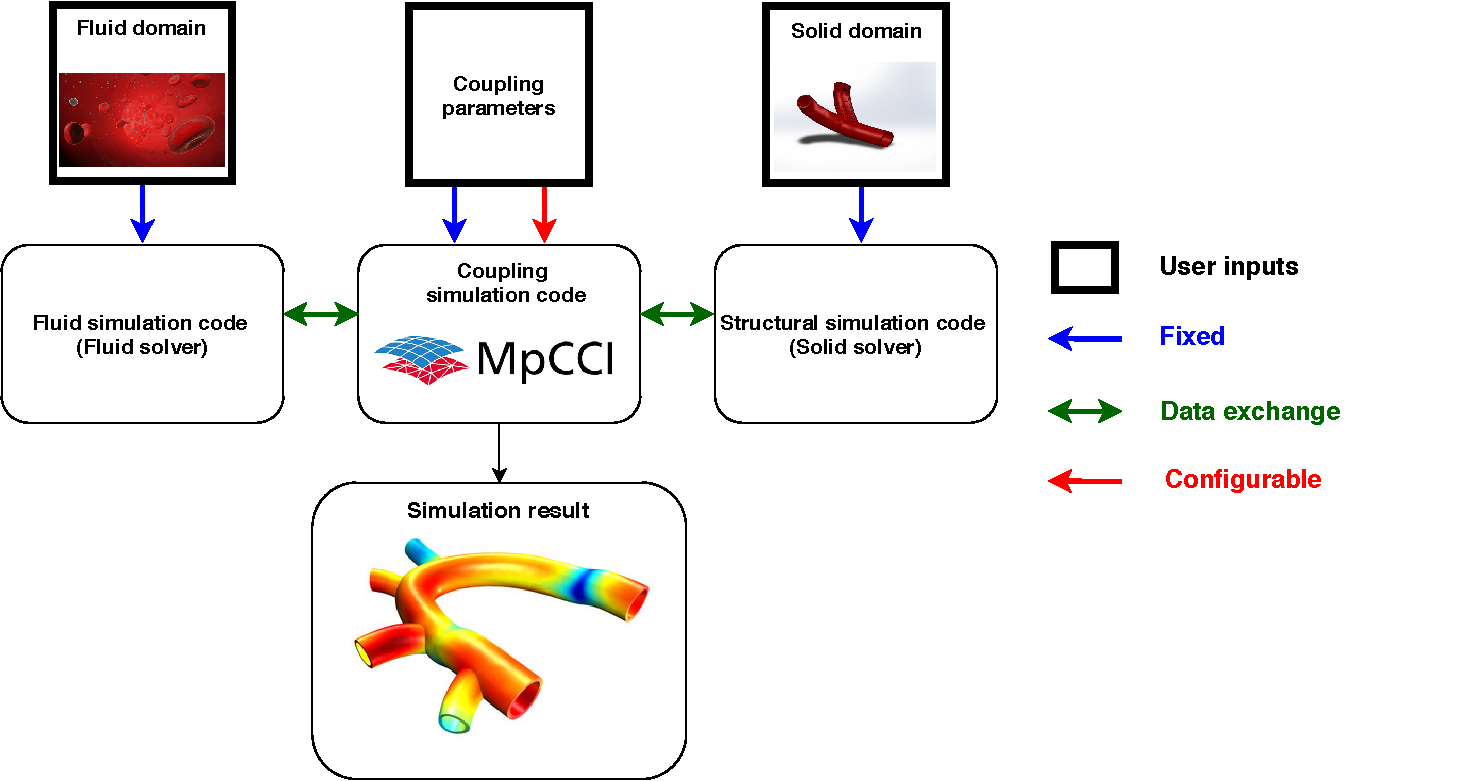
\includegraphics[width=\textwidth, height=0.7\textheight]{images/Coupled_simulation-new.pdf}
		\captionsetup{justification=justified,margin=0.2cm}
		\caption{Multiphysics simulation with a coupling tool. MpCCI - Mesh-based parallel Code Coupling Interface. Images adapted from \cite{Blood-vessel} \cite{blood} \cite{vessel}.}
\end{figure}
\end{frame}

% \footnote{\tiny The fluid domain, solid domain and simulation result images are from \cite{Blood-vessel} \cite{blood} \cite{vessel}.\\}
% \begin{frame}{Objective}
% \begin{itemize}[(I)]
% \justifying
% \item <1- >Improve the robustness and acceleration of the \color{red}multiphysics simulation coupling tool\color{black}, Mesh-based parallel Code Coupling Interface (MpCCI) developed by the Fraunhofer Institute for Algorithms and Scientific Computing (SCAI).
% \newline
% \item <2- >Assist the user by automatically configuring the parameters of the coupling tool.
% \newline
% \item <3- >This study primarily focus on configuring the coupling tool for Fluid-Structure Interaction (FSI) multiphysics simulation studies.
% \end{itemize}
% \end{frame}
\subsection{Problem statement}
\begin{frame}[t]{Problem statement}
% What is the problem? Why is it a problem?
\begin{itemize}
\item<1-> Manually fine-tuning coupling tool parameters is tedious and time-consuming.
\newline
\begin{itemize}
\item Numerous configurable parameters (approximately 15 parameters).
\newline
\item Different types of configurable parameters.
\newline
\item Parameters exhibit forbidden and conditional dependencies.
\newline
\end{itemize}
% \item <2- >\textbf{Goal:} Automatically suggest parameter configuration with lesser runtime than default configuration.
% \newline
% \begin{itemize}
%     \item Automatically configure the parameters of the coupling tool.
%     \newline
%     \item Reduce the simulation runtime relative to the current default parameters.
% \end{itemize}
\end{itemize}
\end{frame}

\subsection{Motivation}
\begin{frame}[t]{Motivation}
% Why is it relevant
% Start with the example of coupling tool parameters
\begin{itemize}
\item <1- > Co-simulation setting up procedure.
\newline
\begin{itemize}
\item No assistance to set coupling parameters for FSI simulations. 
\newline
% \item A single simulation instance to study the aerodynamics of aircraft extends upto weeks.
\item One simulation to study aerodynamics of aircraft $\implies$ upto weeks \cite{aerodynamics_time} \cite{EGO_Basepaper}.
\newline
% \item Development of efficient designs includes repeatedly testing various designs in a robust environment to save time and resources.
\item Repeated testing with numerous designs demands a robust coupling tool.
\newline
\end{itemize}
\item <2- >Coupling tool users.
\begin{columns}[T] % align columns
\begin{column}{.32\textwidth}
\begin{itemize}
    \item Cambridge University
    \newline
    \item CERN
    \newline
    \item Universität Bonn
\end{itemize}
\end{column}%
\hfill%
\begin{column}{.4\textwidth}

\begin{itemize}
    \item Airbus
    \newline
    \item Daimler
    \newline
    \item Volkswagen
    
\end{itemize}
\end{column}%
\end{columns}

\end{itemize}
\end{frame}



\section{Proposed strategy}

\begin{frame}[t]{Proposed solution}


\begin{itemize}
    \item Automatically predict coupling tool parameter configurations.
    \newline
    \item Configurations with relatively lesser runtime than default configuration.
\end{itemize} 
\begin{figure}[h!]
\centering
\includegraphics[width=\linewidth]{images/proposedstrategy_gen.jpg}
% \caption{A simplified illustration of the proposed solution.}
\label{fig:simplegoal}
\end{figure}  
    
\end{frame}

\begin{frame}[t, noframenumbering]{Proposed solution}

\begin{itemize}
    \item Automatically predict coupling tool parameter configurations.
    \newline
    \item Configurations with relatively lesser runtime than default configuration.
\end{itemize} 
\begin{figure}[h!]
\centering
\includegraphics[trim={0 3cm 0 0},width=\linewidth]{images/proposedstrategy_challenge.jpg}
\caption{Proposed solution with challenges. Red markings indicate the challenges.}
\label{fig:simplegoal_challenge}
\end{figure}  
    
\end{frame}


\begin{frame}[t]{Simulation problem and features}
\begin{itemize}
\item FSI simulation problems: 3D driven cavity and elastic flap.
\begin{figure}[!ht]
        \centering
        \begin{subfigure}{.45\textwidth}
          \centering
          \includegraphics[trim={6.5cm 5cm 5.3cm 7cm},clip,width=1.28\linewidth]{images/drivencavity.pdf}
          \caption{2D cross section of 3D driven cavity.}
    \end{subfigure}%
    \begin{subfigure}{.49\textwidth}
          \centering
          \includegraphics[width=1\linewidth, height=0.59\linewidth]{images/elasticflap_geometry.png}
          \caption{ Elastic flap (Dimension in meter).}
    \end{subfigure}
        \caption{Geometry of the simulation problems \cite{MpCCI_documentation}.}
        \label{Fig:simulation_problem}
    \end{figure}
\item Features: Fluid density, fluid viscosity, solid elasticity, Poisson's ratio and solid-fluid density ratio (based on \cite{FSI_properties} \cite{FSI_properties2}).
\newline
\item Each simulation instance of a problem has different feature values.
\end{itemize}
\end{frame}

% \begin{frame}{Simulation instances}
% \begin{itemize}
% \item A python-based package, 'Feature reader', to extract features from the solver and coupling tool files. The files are the configuration and log files.
% \begin{figure}[h!]
% \centering
% \includegraphics[width=0.76\linewidth, height=0.5\textheight]{images/example_feature.png}
% \caption{An example feature fluid viscosity (nu) from the fluid solver configuration file. }
% \end{figure}  
% \end{itemize}
% \end{frame}


\begin{frame}[t]{Proposed solution}

\begin{itemize}
    \item Automatically predict coupling tool parameter configurations.
    \newline
    \item Configurations with relatively lesser runtime than default configuration.
\end{itemize} 
\begin{figure}[h!]
\centering
\includegraphics[trim={0 3cm 0 0},width=\linewidth]{images/proposedstrategy_challenge2a.jpg}
% \caption{Proposed solution with challenges.}
\label{fig:simplegoal_challenge2}
\end{figure}  
    
\end{frame}

\begin{frame}{Hyperparameters of the coupling tool}
\small
% \begin{itemize}
% \item The configuration space, $\Theta$: Vector space spanned by the hyperparameters.
% \end{itemize}
\begin{table}[htbp]
\footnotesize
\begin{center}
\begin{tabular}{|l|l|l|}
\hline
\textbf{Parameter, P} & \textbf{Parameter type} & \textbf{Domain of the parameter, D} \\ \hline
Coupling scheme & Categorical &\makecell[l]{\color{brown}Implicit-Transient:Implicit-Transient\color{black},\\Explicit-Transient:Explicit-Transient} \\ \hline
Initial exchange & Categorical & \makecell[l]{exchange:exchange, receive:exchange, \\exchange:receive}  \\ \hline
\color{brown}Relaxation-0 & Categorical & \color{blue}True\color{black}, False \\ \hline
\color{brown}Relaxation-1 & Categorical & \color{blue}True\color{black}, False \\ \hline
\color{blue}Relaxation method & Categorical &\color{green} Quasi-Newton\color{black}, \color{red}Fixed\color{black}, Aitken, \color{magenta}Ramping \\ \hline
\color{green}Anderson mix& Categorical & Least squares, Standard, Inverse \\ \hline
\color{green}Number of levels  & Integer & [0, 16] \\ \hline
\color{green}Omega & Float & [1e-07, 2.0] \\ \hline
\color{magenta}Ramp-0 & Float & [0.0, 2.0] \\ \hline
\color{magenta}Ramp-d & Float & [0.001,1.0] \\ \hline
\color{red}Relaxation factor & Float & [0.0,2.0] \\ \hline
\end{tabular}
\end{center}
\caption{Hyperparameters of the tool. The coloring represents the existence of the parameter, P only if the respective color is selected in domain, D for all the preceding parameter.}
\label{table:parametertypes}
\end{table}
\end{frame}{}



\subsection{Dataset generation}
\begin{frame}{Dataset generation}
\begin{figure}[h!]
\centering
\includegraphics[width=\linewidth]{images/Optimizationphase_new.jpg}
\caption{Dataset generation overview. \textbf{Cost of each instance is the simulation runtime (in seconds)} for the respective parameter configuration.}
\end{figure}  
\end{frame}


\subsection{Sequential Model-based Algorithm Configuration (SMAC)}
\begin{frame}[t]{Optimization: Sequential Model-based Algorithm Configuration (SMAC)}

\begin{itemize}
\item Random Forest (RF) surrogate\footnote{surrogate - substitute. A model mimicking the coupling tool.} and acquisition function\footnote{To select next promising point for evaluation on the target algorithm.\\}.
%  The model aids in performing fewer direct evaluations of the target algorithm.
\newline
\item Expected Improvement (EI) - how promising is a configuration depending on the model constructed?
\newline
\item <2- > \textbf{Why SMAC?}
\newline
\begin{itemize}
\item RF better surrogate model on data with categorical parameters \cite{Hutterphd} \cite{SMAC_mainpaper}.
\newline
\item State of the art optimization algorithm \cite{SMAC_ParamILS_GGA_compare}.
% \newline
% \item Supports numerical, categorical and conditional parameters \cite{SMAC_mainpaper}. % \item Supports forbidden configurations \cite{SMAC_mainpaper}.
\end{itemize}
\end{itemize}
\end{frame}

% \begin{frame}[t]{SMAC Good-Bad-Ugly configurations}

% \begin{columns}[T] % align columns
% \begin{column}{.6\textwidth}
% \begin{figure}[!ht]
% \centering
% \includegraphics[width=\linewidth]{images/Good_bad_ugly_cost.pdf}
% \captionsetup{justification=justified}
% \caption{An illustration of good-bad-ugly configurations for single instance optimization over 100 iteration.}
% \label{fig:good-bad-ugly}
% \end{figure}
% \end{column}%
% \hfill%
% \begin{column}{.4\textwidth}
% \begin{itemize}
%     \item <2- >Bad $\implies$ crashed simulation.
%     \newline
%     \item <2- >Good and ugly $\implies$ successful simulation.
%     \newline
%     \item <3- >Ugly $\implies$ outliers of the successful simulation distribution. 
% \end{itemize}
% \end{column}%
% \end{columns}
% \end{frame}

\begin{frame}[t]{Proposed solution}

\begin{itemize}
    \item Automatically predict coupling tool parameter configurations.
    \newline
    \item Configurations with relatively lesser runtime than default configuration.
\end{itemize} 
\begin{figure}[h!]
\centering
\includegraphics[trim={0 3cm 0 0},width=\linewidth]{images/proposedstrategy_challenge3a.jpg}
% \caption{Proposed solution with challenges.}
\label{fig:simplegoal_challenge3}
\end{figure}  
    
\end{frame}

\subsection{Training procedure}
\begin{frame}[t]{Training and prediction}
\begin{itemize}
\item Trained two types of models (blue indicate the differences).
\begin{itemize}
  \item Cost response model
  \item Configuration response model
% \tikz\node[opacity=0.2,align=left,inner xsep=0pt]
% {%
%   \parbox[t]{\linewidth}{%

%   \item Configuration response model}%
% };
\end{itemize}
\end{itemize}
\begin{columns}[T] % align columns
\begin{column}{.5\textwidth}
\begin{figure}[!ht]
\centering
\includegraphics[width=\linewidth]{images/cost_response_new.jpg}
\captionsetup{justification=justified}
% \caption{Cost response model.}
\label{fig:cost_new1}
\end{figure}
\end{column}%
\hfill%
\begin{column}{.5\textwidth}
\end{column}%
\end{columns}
\end{frame}

\begin{frame}[t, noframenumbering]{Training and prediction}

\begin{itemize}
\item Trained two types of models (blue indicate the differences).
\begin{itemize}
  \item Cost response model
  \item Configuration response model
\end{itemize}
\end{itemize}


\begin{columns}[T] % align columns
\begin{column}{.5\textwidth}
\only{\begin{figure}[!ht]
\centering
\includegraphics[width=\linewidth]{images/cost_response_new.jpg}
\captionsetup{justification=justified}
% \caption{Cost response model.}
\label{fig:cost_new2}
\end{figure}}
\end{column}%
\hfill%
{\begin{column}{.5\textwidth}
\begin{figure}[!ht]
\centering
\includegraphics[width=\linewidth]{images/configuration_response_new.jpg}
\captionsetup{justification=justified}
% \caption{Configuration response model.}
\label{fig:config_new}
\end{figure}
\end{column}}%
\end{columns}
\end{frame}


\section{Experiments and results}

\begin{frame}[t]{SMAC vs Default}
\begin{itemize}
    \item Does SMAC configurations perform better than the default configurations?
    \newline
    \item Mean percentage decrease in runtime: 24.92\%
    \end{itemize}
\begin{figure}
  \begin{columns}
    \column{.6\linewidth}
    \includegraphics[width=\linewidth, height=0.58\textheight]{images/SMAC_vs_default.pdf}
    \column{.4\linewidth}
    \caption{The runtime for each instance is normalized with the SMAC best configuration runtime. $\infty$ denote cost of crashed simulations.}
  \end{columns}
\end{figure}
\end{frame}

\begin{frame}[t]{Model selection across cost transformations}

\begin{itemize}
    \item 5-fold Cross Validation (CV) with Root Mean Square Error (RMSE). 
    \newline
    \item \textbf{Similar trend is observed in configuration response model.}
    \newline
\end{itemize}
\begin{figure}[!ht]
\centering
\begin{subfigure}{.45\textwidth}
\centering
\includegraphics[width=\linewidth]{images/rmse-cost_1.pdf}
% \caption{Rank 1 for cost response model.}
\end{subfigure}
\begin{subfigure}{.45\textwidth}
\centering
\includegraphics[width=\linewidth]{images/rmse-cost_0.pdf}
% \caption{Rank 2 for cost response model.}
\end{subfigure}
\caption{\textbf{Lower RMSE is better.} Models - Random forest (RF), K- Nearest Neighbors (KNN), Support Vector Machine (SVM), Gradient Boosting (GB), Quantile Random Forest (QRF), Random Forest predicting EI (RF\_EI).}
\label{Fig:modelselection_compare}
\end{figure}
\end{frame}{}

\begin{frame}[t]{Evaluation on simulation instances}
\begin{itemize}
\item No benchmarks to compare the parameter configuration performance. 
\newline
\item SMAC best configuration runtime is used to compare the models.
\newline
\item Normalized Runtime (NR) of a configuration from model 'X'.
\newline
\begin{equation}
\small
\text{NR} = \frac{\text{Runtime of the configuration from 'X'}}{\text{Runtime of the best configuration from SMAC}}  
\label{equation:normalized}
\end{equation}
\newline
\item Average Normalized Runtime (ANR) of configurations from model 'X'.
\begin{equation}
\small
\begin{split}
\text{ANR} = \frac{\sum_{i=1}^{N} \text{{NR of a configuration from 'X' on instance i}}}{N}
\label{equation:averagenormalized}
\end{split}
\end{equation}
\newline
\end{itemize}
\end{frame}

\begin{frame}[t]{Evaluation on simulation instances}
\begin{figure}[!ht]
\centering
\includegraphics[width=\linewidth]{images/final-eval-new.pdf}
\captionsetup{justification=justified,margin=0.2cm}
\caption{\textbf{Lower value is the better model}. The parameter configuration predicted by the top three models with less ANR is suggested by the smart coupling tool.}
\label{fig:training_prediction}
\end{figure}
\end{frame}

\begin{frame}[t]{Model performance on a crashed simulation instance}

\begin{itemize}
\item Positive impact of the smart coupling tool suggested configurations.
\end{itemize}
\begin{figure}
  \begin{columns}
    \column{.6\linewidth}
    \includegraphics[width=\linewidth, height=0.58\textheight]{images/real-eval-new.pdf}
    \column{.4\linewidth}
    \caption{Default configuration results in crashed simulation. The parameter configurations suggested by these models result in a successful simulation.}
  \end{columns}
\end{figure}
\end{frame}

\section{Conclusion}

\begin{frame}[t]{Contributions}

\begin{itemize}
\item Methodology to predict parameter configurations of a coupling tool for accelerated simulation.
\newline
\item A preliminary multiphysics simulation dataset for machine learning.
\newline
\item Feature reader: To extract features of the simulation instance.
\newline
\item Smart coupling: To suggest parameter configurations to the user given a FSI simulation instance. 
% \item Repeatability of SMAC for optimizing a single multiphysics simulation instance.
\end{itemize}{}
\end{frame}

\begin{frame}[t]{Future work}
    
\begin{itemize}
\item Generate dataset v2.0 and evaluate on additional FSI \& non-FSI problems.
\newline
\item Formalize the feature selection method across problems.
\newline
\item Investigate deep learning based models to suggest parameter configurations.
\newline
\item Compare performance of SMAC with other optimization algorithms.
\newline
\item Explainable artificial intelligence (XAI).
\end{itemize}{}
\end{frame}


\begin{frame}[t, allowframebreaks]
\frametitle{References}
\label{lastpage}
\printbibliography[title={References}]
\end{frame}

\begin{frame}
\begin{center}
\Huge Thank you for your time!
\end{center}{}

\end{frame}

\appendix
\section{Extras}

\begin{frame}[t]{SMAC Good-Bad-Ugly configurations}

\begin{columns}[T] % align columns
\begin{column}{.6\textwidth}
\begin{figure}[!ht]
\centering
\includegraphics[width=\linewidth]{images/Good_bad_ugly_cost.pdf}
\captionsetup{justification=justified}
\caption{An illustration of good-bad-ugly configurations for single instance optimization over 100 iteration.}
\label{fig:good-bad-ugly-last}
\end{figure}
\end{column}%
\hfill%
\begin{column}{.4\textwidth}
\begin{itemize}
    % \item Bad $\implies$ crashed simulation.
    % \newline
    % \item Good and ugly $\implies$ successful simulation.
    \item Difficulty to decide whether the configuration is required for training.
    \newline
    \item GOOD - YES, I want to use it of course.
    \newline
    \item BAD - NO, I definitely do not want you for my training (taking a easy decision of removing them).
    \newline
    \item UGLY - - , I do not know what to do with these configurations at the moment.
\end{itemize}
\end{column}%
\end{columns}
\end{frame}

\begin{frame}{SMAC Good-Bad-Ugly configurations}
\begin{table}[!ht]
\centering
\begin{tabular}{|c|c|}
\hline
\textbf{Configurations} & \textbf{\% of total configurations} \\ \hline
The Good (Optimal and sub-optimal) & 49.2 \\ \hline
The Bad (Crashed) & 47.8 \\ \hline
The Ugly (Below sub-optimal) & 3.0 \\ \hline
\end{tabular}
\captionsetup{justification=justified}
\caption[Percentage of good-bad-ugly configurations from SMAC]{Percentage of good-bad-ugly configurations from SMAC for per-instance optimization (average over 16 instances). The ugly configurations are considered to be the configurations with normalized cost value above the upper inner fence (Q3 + 1.5 $\times$ IQR) of the successful simulations distribution.}
\label{table:configuration_split}
\end{table}
\end{frame}


\begin{frame}{Related work of AAC}
\begin{figure}
\centering
\includegraphics[width=0.6\textwidth]{images/AAC_types.jpg}
\captionsetup{justification=justified,margin=0.2cm}
\caption{AAC methods.}
\end{figure}
\end{frame}

\begin{frame}{Related work of AAC}

\begin{itemize}
\item Traditional methods: Hill-climbing \cite{Gratch_1992}, Beam search \cite{Minton_1993}, Racing methods \cite{FRace_paper} \cite{IFRace_paper}.
\newline
\item Current state-of-the-art: Parameteric-Iterative Local Search (ParamILS) \cite{ParamILS_mainpaper}, Gender-based Genetic Algorithm (GGA) \cite{GGA_paper}, Sequential Model-based Algorithm Configuration (SMAC) \cite{SMAC_mainpaper}.
\newline
\item Deficits:
\begin{itemize}
\item Traditional methods can handle only lesser number of parameters, approximately five \cite{Gratch_1992} \cite{Minton_1993}. In addition, the methods are restricted to only numerical and categorical parameters \cite{AAC_Mainreview}. 
\newline
\item ParamILS is applicable only for configuring algorithms with categorical parameters. It explicitly requires a discretization procedure \cite{ParamILS_mainpaper}.
\newline
\item GGA is computationally expensive involving a fitness function evaluation and supports only per-instance optimization. In addition, fails for complex conditional parameters \cite{SMAC_ParamILS_GGA_compare}.
\end{itemize}
\end{itemize}
\end{frame}

\begin{frame}[t]{Related work of Coupling tool}
\begin{itemize}
    \item preCICE simulation tool, ADVENTURE\_Coupler - Competitor coupling tool \cite{FSI_Bungartz}.
    \newline
    \item No means of automatically estimating the optimal parameter values of the coupling tools \cite{FSICartesiangrid}.
\end{itemize}
\end{frame}


\begin{frame}[t]{Related work/Application of SMAC}
\begin{itemize}
\item Mixed integer programming \cite{SMAC_mainpaper}.
\item Boolean satisfiability problem (SAT)\footnote{SAT is the problem of determining if there exists an interpretation that satisfies a given Boolean formula\\} \cite{SMAC_mainpaper}.
\item Hyperparameter optimization \cite{hponn}.
\item Robot localization \cite{OscarLima_SMAC}.
\end{itemize}
\end{frame}

\begin{frame}[t]{Why SMAC?}

% \item Model-based methods perform lesser direct evaluations of the target algorithm to find the optimal parameter configuration by making use of the knowledge from the previous evaluations.

\begin{itemize}
\item Advantages of SMAC \cite{SMAC_mainpaper} \cite{Hutterphd}:
\begin{itemize}
\item Model-based AAC method.
% attempt to recognise and benefit from regularities in a given configuration space.
\item RF surrogate model performs better with categorical parameters \cite{Hutterphd} \cite{SMAC_mainpaper}.
\item Configures numerical, categorical and conditional parameters \cite{SMAC_mainpaper}. 
\item SMAC supports forbidden configurations \cite{SMAC_mainpaper}.
\item Surrogate model aids in performing fewer direct evaluations of the target algorithm \cite{BayesianOptimization_papertutorials}.
\newline
\end{itemize}

\item Comparative study between ParamILS, GGA and SMAC for configuring Boolean satisfiability problem (SAT) solvers\footnote{SAT is the problem of determining if there exists an interpretation that satisfies a given Boolean formula\\} illustrate \color{red} SMAC is better in algorithm configuration with respect to solution quality and runtime \color{black}\cite{SMAC_ParamILS_GGA_compare}. 

\end{itemize}
\end{frame}{}

\begin{frame}{SMAC steps}

\begin{figure}
\centering
\includegraphics[width=\textwidth]{images/SMAC_simplified_new.jpg}
\captionsetup{justification=justified,margin=0.2cm}
\caption{A simplified illustration of SMAC.}
\end{figure}
    
\end{frame}

\begin{frame}[t]{Why log-transformation better than normal?}

\begin{itemize}
\item Pre-processed cost metric - transformed using the shown transformations and normalized to fix the minimum/ best cost metric at 1.  
    
\begin{table}[!h]
\centering
\begin{tabular}{|l|l|l|}
\hline
\multicolumn{1}{|c|}{\multirow{2}{*}{\textbf{Transformation}}} & \multicolumn{2}{c|}{\textbf{Pre-processed cost metric}} \\ \cline{2-3} 
\multicolumn{1}{|c|}{} & \multicolumn{1}{c|}{\textbf{Skewness}} & \multicolumn{1}{c|}{\textbf{Standard deviation}} \\ \hline
LOG & \color{green}0.2152 & \color{green}0.6718\\ \hline
LOG-SCALED & -1.036 & 7.417 \\ \hline
INVERSE & -1.532 & 2501 \\ \hline
NONE & \color{red}\textbf{6.331} & \color{red}\textbf{3304} \\ \hline
\end{tabular}
\captionsetup{justification=justified}
\caption[Statistical measures of the pre-processed cost metrics]{Statistical measures of the pre-processed cost metrics using different transformations. The green and red highlights indicate the first and last ranked statistical values, respectively, across different transformations.}
\label{table:skewness}
\end{table}

\end{itemize}
\end{frame}

\begin{frame}[t]{Lessons learned}
\begin{itemize}
\item Sort out patterns in failed simulations for dataset generation using ML approaches.
\item Data normalization.
\item Test cases for the input batch provider.
\item Test cases for simple implementations and then proceed for higher dimensional regression. To avoid the black box issue.
\end{itemize}
\end{frame}


\begin{frame}[t]{How did you choose the training models?}
\begin{itemize}
\item RF, GB performs well on categorical data.

\item SATZILLA \cite{SATZILLA} one of the related works of SMAC utilize KNN and SVM.

\item In future have to include different models. 

\item SATZILLA paper. This paper uses these models to predict the runtime to select the best solver to solve a particular problem instance in SAT solvers.

\item SOLVER uses different algorithms to solve different problems.

\item SOLVER parameters are pre-configured by AAC algorithms like SMAC, ParamILS.

\item So dataset to train: solver name- instance - runtime. 

\item This is parallel to our domain of application- Algorithm selection.
	
\end{itemize}
\end{frame}{}

\begin{frame}[t]{How can you tell the parameter you find are optimal?}

\begin{itemize}
\item We cannot practically guarantee optimal parameters in SMAC. SMAC convergence to optimal theorem is provided in \cite{SMAC_extendedpaper}. However, we should do intensification with infinte time.

\item We have said SMAC suggests a best configuration repeatably with a particular cost value.

\item But, the best configurations from SMAC are considered optimal/best for a particular instance for evaluating the predicted configurations effectiveness.

\item At the end, the deviation from the best is given as a suboptimal configuration.

\item Convergence doesnt mean optimal solution is obtained.

\end{itemize}
\end{frame}

\begin{frame}[t]{Repeatability of SMAC}

\begin{itemize}
\item \textbf{Test:} Is SMAC repeatable in finding the best configuration of a simulation instance?
\newline
\item \textbf{Oneliner:} Find repeatability co-efficient of SMAC by optimizing a simulation instance using SMAC for 3 trials.
\newline
\item \textbf{Motive:} Important to know the consistency of SMAC to rely on the configurations provided by SMAC. It gives a measure of uncertainity associated with a particular configuration.
\end{itemize}
    
\end{frame}

\begin{frame}{Repeatability of SMAC}

\begin{table}[htbp]
\begin{tabular}{|c|c|c|c|r|r|}
\hline
\multicolumn{ 1}{|c|}{\textbf{Instance}} & \multicolumn{3}{|p{4.5cm}|}{\centering \textbf{Best cost from\\ SMAC (seconds)}} & \multicolumn{1}{|p{2cm}|}{\centering \textbf{Average\\ cost (seconds)}}  & \multicolumn{1}{|p{2cm}|}{\centering \textbf{Standard\\ deviation\\(seconds)}}  \\ \cline{ 2- 4}
\multicolumn{ 1}{|c|}{} & \textbf{Trial 1} & \textbf{Trial 2} & \textbf{Trial 3} & \multicolumn{ 1}{l|}{} & \multicolumn{ 1}{l|}{} \\ \hline
1 & 399.84 & 397.82 & 396.41 & 398.02 & 1.72 \\ \hline
2 & 545.76 & 520.97 & 520.60 & 529.11 & 14.42 \\ \hline
3 & 403.16 & 393.68 & 416.12 & 404.32 & 11.26 \\ \hline
4 & 465.79 & 452.49 & 467.15 & 461.81 & 8.09 \\ \hline
5 & 2019.46 & 2026.78 & 2011.49 & 2019.24 & 7.64 \\ \hline
6 & 724.22 & 726.98 & 744.65 & 731.95 & 11.08 \\ \hline
\end{tabular}
\captionsetup{justification=justified}
\caption{Average cost and standard deviation for the simulation instances involved in repeatability test of SMAC. Each trial involves 100 iterations of SMAC}
\label{table:smac_repeatability}
\end{table}
    
\end{frame}

\begin{frame}[t]{Repeatability coefficient}

\begin{itemize}
\item Repeatability coefficient: The maximum deviation with a probability of 95\% between two successive measurements of the same subject under same measurement conditions and using the same procedure \cite{repeatability1} \cite{repeatability2}.
\newline
\item $S_r = 1.96 \times \sigma$ , where $\sigma$ is the mean standard deviation of the simulation instance costs (within group standard deviation).
\end{itemize}
\begin{table}[]
\centering
\begin{tabular}{|l|l|}
\hline
\textbf{Metric} & \textbf{Value} \\ \hline
\begin{tabular}[c]{@{}l@{}}Mean variation in run-time\\  within simulation instances ($MS_w$)\end{tabular} & 97.46 seconds \\ \hline
Repeatability coefficient ($S_r$) & 19.34 seconds \\ \hline
\end{tabular}
\captionsetup{justification=justified}
\caption{Repeatability of SMAC}
\label{table:experiment3_metrics}
\end{table}
    
\end{frame}


% \begin{frame}{Experiment 4- SMAC Good-Bad-Ugly ratio}
% \begin{itemize}
% \item Test: Does SMAC find many good configurations to enrich the dataset with more good configurations? 
% \newline
% \item Oneliner: Run SMAC for an instance and analyze the runhistory of SMAC.
% \newline
% \item Motive: The requirement of more good configurations and less variance in the dataset. This increases the quality of the dataset.
% \end{itemize}
% \end{frame}


\begin{frame}[t]{Behavior of SMAC with respect to iteration count}

\begin{itemize}
\item \textbf{Test:} How many iterations is required for SMAC to find better configurations? 
\newline
\item \textbf{Oneliner:} Run SMAC with different iteration count and estimate the best cost identified by SMAC. 
\newline
\item \textbf{Motive:} Aids in identifying the number of times the target algorithm has to be evaluated by SMAC.
\end{itemize}

\end{frame}

\begin{frame}{Behavior of SMAC with respect to iteration count}

\begin{figure}[!ht]
\centering
\includegraphics[width=0.8\linewidth, height=0.7\textheight]{images/Iteration_vs_cost.pdf}
\captionsetup{justification=justified}
\caption{SMAC best cost versus number of iterations. The ability to find good configurations increases with iteration count.}
\label{fig:experiment3_results}
\end{figure}

\end{frame}

\begin{frame}{Explainable AI idea}

\begin{itemize}
\item Feature importance of each Out-Of-Bag (OOB) data using RMSE.
\item Learn which feature leads to successful and crashed.
\item Intermediate studies: SVM-RBF classifies with an accuracy of 95\% (approx).
\end{itemize}
    \begin{figure}[!ht]
        \centering
      \begin{subfigure}{.5\textwidth}
          \centering
          \includegraphics[width=\linewidth]{images/pca.pdf}
          \caption{PCA.}
    \end{subfigure}%
     \begin{subfigure}{.5\textwidth}
          \centering
          \includegraphics[width=\linewidth]{images/tsne.pdf}
          \caption{t-SNE.}
    \end{subfigure}
        \caption{Successful vs crashed simulations. Includes optimization and random generation.}
        \label{Fig:explainableAI}
    \end{figure}
\end{frame}

\begin{frame}{Dataset generation difficulty}

\begin{itemize}
\item Configuration fixed, features varied (eitherwise).
\item Possible reasons: Feature values bounds, or bad default configurations.
\item Features are highly overlapping. Manually finding feature and configuration values that lead to successful simulation for generating dataset is difficult.
\end{itemize}
    \begin{figure}[!ht]
        \centering
      \begin{subfigure}{.5\textwidth}
          \centering
          \includegraphics[width=\linewidth]{images/pca.pdf}
          \caption{PCA.}
    \end{subfigure}%
     \begin{subfigure}{.5\textwidth}
          \centering
          \includegraphics[width=\linewidth]{images/tsne.pdf}
          \caption{t-SNE.}
    \end{subfigure}
        \caption{Successful vs crashed simulations. Includes optimization and random generation.}
        \label{Fig:dataset_challenge}
    \end{figure}

\end{frame}


\begin{frame}{Significance of hyperparameters}

\begin{figure}[!ht]
\centering
\includegraphics[width=\textwidth]{images/driven_cavity_result1.png}
\captionsetup{justification=justified}
\caption[An illustration of the significance of hyperparameters]{Impact of 'Coupling scheme' hyperparameter in driven cavity- Iterative transient coupling versus explicit coupling for 3D driven cavity \cite{MpCCI_documentation}. The simulation will fail on configuring the coupling scheme with explicit coupling.}
\label{Fig:iterative_vs_explicit}
\end{figure}
\end{frame}
\begin{frame}{Significance of hyperparameters}
\begin{figure}[!h]
\centering
\includegraphics[trim={0 3cm 0 3cm},clip,width=0.5\textwidth,height=0.65\textheight]{images/qn_relaxation_drivencavity_1.pdf}
\captionsetup{justification=justified}
\caption[Effectiveness of Quasi-Newton relaxation method for 3D-driven cavity]{Effectiveness of Quasi-Newton relaxation method for 3D-driven cavity \cite{MpCCI_documentation}.}
\label{Fig:qn_relaxation}
\end{figure}

\end{frame}


\begin{frame}{Default values for the hyperparameters}
\begin{itemize}
    \item  In FSI, Quasi-Newton (QN) is the most efficient and robust relaxation method for partitioned coupling \cite{robustqn} \cite{robustqn2}. 
    \item The following default parameter values are used in MpCCI for QN based problems.
    
\begin{table}[htbp]
\begin{center}
\begin{tabular}{|l|l|}
\hline
\textbf{Parameter, P} & \textbf{Default value} \\ \hline
Coupling scheme & Implicit-Transient:Implicit-Transient\\ \hline
Initial exchange & receive:exchange \\ \hline
Relaxation\_0 & False  \\ \hline
Relaxation\_1 & True  \\ \hline
Relaxation method & Quasi-Newton \\ \hline
Andersonmix type & Inverse  \\ \hline
Number of levels  & 1 \\ \hline
Omega & 0.1  \\ \hline
Ramp\_0 & 0.1 \\ \hline
Ramp\_d & 0.1 \\ \hline
Relaxation factor & 0.1 \\ \hline
\end{tabular}
\end{center}
\captionsetup{justification=justified}
\caption[Default parameter configuration of MpCCI]{Default configuration majorly used in MpCCI.}
\label{table:parameterdefaultvalues}
\end{table}

\end{itemize}

\end{frame}

\begin{frame}{Bayesian Optimization (BO)}

\begin{itemize}

\item BO with Gaussian Process surrogate model \cite{martin_bo_tutorial}.
    
\begin{figure}[!ht]
\centering
\includegraphics[width=\linewidth]{images/BO_objective.png}
\captionsetup{justification=justified}
\caption[An example objective function under BO]{An example objective function to illustrate the working of Bayesian optimization.}
\label{fig:BO_objective}
\end{figure}

\end{itemize}

\end{frame}

\begin{frame}{BO}
    
    \begin{figure}[!ht]
		\centering
		\begin{subfigure}{1\textwidth}
  			\centering
  			\includegraphics[scale=0.226]{images/BO1.png}
  			\caption{Evaluate the query points (EVALUATE) $\rightarrow$Fit surrogate to initial evaluation (FIT)$\rightarrow$ Maximize EI to find the next query point (MAXIMIZE EI).}
  			\label{fig:BO1}
		\end{subfigure}
		\begin{subfigure}{1\textwidth}
  			\centering
  			\includegraphics[scale=0.226]{images/BO2.png}
  			\caption{EVALUATE $\rightarrow$ FIT $\rightarrow$ MAXIMIZE EI.}
  			\label{fig:BO2}
		\end{subfigure}
\captionsetup{justification=justified}
\caption[Illustration of BO- Iterations 1 to 4.]{Illustration of BO- Iterations 1 and 2.}
\label{fig:BO_steps1}
\end{figure}

\end{frame}


\begin{frame}{BO}
    \begin{figure}[!ht]
		\centering
		\begin{subfigure}{1\textwidth}
  			\centering
  			\includegraphics[scale=0.238]{images/BO3.png}
  			\caption{EVALUATE $\rightarrow$ FIT $\rightarrow$ MAXIMIZE EI.}
  			\label{fig:BO3}
		\end{subfigure}
		
	\begin{subfigure}{1\textwidth}
  			\centering
  			\includegraphics[scale=0.238]{images/BO4.png}
  			\caption{EVALUATE $\rightarrow$ FIT $\rightarrow$ MAXIMIZE EI.}
  			\label{fig:BO4}
		\end{subfigure}
		
\captionsetup{justification=justified}
\caption[Illustration of BO- Iterations 1 to 4.]{Illustration of BO- Iterations 3 and 4.}
\label{fig:BO_steps2}
\end{figure}
\end{frame}

\begin{frame}{BO}
        \begin{figure}[!ht]
		\centering

	\begin{subfigure}{1\textwidth}
  			\centering
  			\includegraphics[scale=0.238]{images/BO5.png}
  			\caption{EVALUATE $\rightarrow$ FIT $\rightarrow$ MAXIMIZE EI.}
  			\label{fig:BO5}
		\end{subfigure}
		\begin{subfigure}{1\textwidth}
  			\centering
  			\includegraphics[scale=0.238]{images/BO6.png}
  			\caption{EVALUATE $\rightarrow$ FIT $\rightarrow$ MAXIMIZE EI.}
  			\label{fig:BO6}
		\end{subfigure}
	
\captionsetup{justification=justified}
\caption[Illustration of BO- Iterations 1 to 4.]{Illustration of BO- Iterations 5 and 6.}
\label{fig:BO_steps3}
\end{figure}
\end{frame}

\begin{frame}{BO}

    \begin{figure}[!ht]
		\centering
		\begin{subfigure}{1\textwidth}
  			\centering
  			\includegraphics[scale=0.238]{images/BO7.png}
  			\caption{EVALUATE $\rightarrow$ FIT $\rightarrow$ MAXIMIZE EI.}
  			\label{fig:BO7}
		\end{subfigure}
		
	\begin{subfigure}{1\textwidth}
  			\centering
  			\includegraphics[scale=0.238]{images/BO8.png}
  			\caption{EVALUATE $\rightarrow$ FIT $\rightarrow$ MAXIMIZE EI. BO terminates returning the best sample point for 8 iterations.}
  			\label{fig:BO8}
		\end{subfigure}
	
\captionsetup{justification=justified}
\caption[Illustration of BO- Iterations 1 to 4.]{Illustration of BO- Iterations 7 and 8.}
\label{fig:BO_steps4}
\end{figure}
    
\end{frame}




\begin{frame}{Proposed strategy: Overview}

\begin{figure}[h!]
\centering
\includegraphics[width=1\linewidth,height=0.7\textheight]{images/Processflow.jpg}
\caption{Overview of the proposed strategy to predict optimal parameter configuration. The color resemblances between the online and offline parts of the pipeline illustrate the usage of the same machine learning model, similar feature extraction method and similar input simulation problem.}
\label{fig:proposedsolution}
\end{figure}  
	
\end{frame}

\end{document}

% https://homes.cs.washington.edu/~mernst/advice/giving-talk.html


% \begin{frame}{Training and Prediction}
%     \begin{figure}[!ht]
%         \centering
%       \begin{subfigure}{.5\textwidth}
%           \centering
%           \includegraphics[width=\linewidth]{images/configuration_response.jpg}
%           \caption{Configuration response model.}
%     \end{subfigure}%
%      \begin{subfigure}{.5\textwidth}
%           \centering
%           \includegraphics[width=\linewidth]{images/cost_response.jpg}
%           \caption{Cost response model.}
%     \end{subfigure}
%         \caption{Training machine learning models to predict coupling tool parameter configuration.}
%         \label{Fig:traintypes}
%     \end{figure}

% \end{frame}

% TIP: 6 experiments testing the various parts of the proposed approach and finally evaluation of the configurations predicted by the proposed approach.
% \begin{frame}{SMAC best versus default configuration}
% \begin{itemize}
% \item Test: Is SMAC able to find configurations better than the default configurations?
% \newline
% \item Oneliner: Runtime of SMAC best configuration\footnote{\tiny Sub-optimal configuration over 100 iterations of SMAC.\\} is compared against the default configuration runtime.
% \newline
% \item Motive: Need for configurations better than default configuration in the dataset.
% \end{itemize}
% \end{frame}

% \begin{frame}{Model selection}
% \begin{itemize}
% \item Models considered for selection are provided below. 
% \begin{table}[!ht]
% \verysmall
% \centering
% \begin{tabular}{|c|c|}
% \hline
% \textbf{Model notation} & \textbf{Model name} \\ \hline
% RF & Random Forest \\ \hline
% GB & Gradient Boosting \\ \hline
% SVM & Support Vector Machine \\ \hline
% QRF & Quantile Random Forest \\ \hline
% KNN & K- Nearest Neighbors \\ \hline
% \multirow{2}{*}{RF\_EI} & \multirow{2}{*}{\begin{tabular}[c]{@{}c@{}}Random Forest predicting\\ EI\footnote{Cost response model with cost metric, EI of a configuration.\\}\end{tabular}} \\
%  &  \\ \hline
% \end{tabular}
% \captionsetup{justification=justified}
% \caption[Notation of machine learning models used for training]{Different configuration and cost response models used for model selection \cite{SATZILLA}.}
% \label{table:modelname}
% \end{table}
% \item 5-fold cross validation (CV) with Root Mean Square Error (RMSE).
% \newline
% \item Normalized runtime (cost metric) is transformed using logarithmic and none transformation.
% \end{itemize}
% \end{frame}{}

% \begin{frame}{Background}
% \begin{itemize}
% \item This problem of automatically configuring the parameters of a algorithm or process falls under the research domain of Automated Algorithm Configuration (AAC). 

% \begin{figure}
% 		\centering
% 		\includegraphics[width=0.9\textwidth]{images/AC_workflow.png}
% 		\captionsetup{justification=justified}
% 		\caption{Automated Algorithm configuration workflow \cite{Pitfalls}. The target algorithm $\mathcal{A}$ is evaluated with different \color{red}parameter configurations $\theta$ \color{black} on various \color{red}instances $\pi$ \color{black} of the problem. The cost metric of the evaluation $c(\theta,\pi)$ is provided to the configurator. The popular cost metric are time taken to solve the instance or solution quality.}
% \end{figure}

% \end{itemize}
% \end{frame}